\chapter{【不多看一眼】}


\begin{wrapfigure}{r}{0.3\textwidth}
\centering
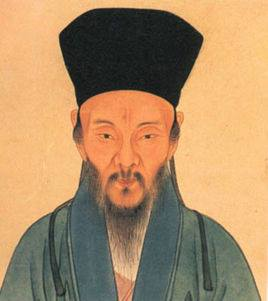
\includegraphics[width=0.3\textwidth]{pics/p001.jpg}
\vspace{-25pt}
\caption{王守仁}
%\label{test}
\end{wrapfigure}

文/喬凱凱
\footnote{摘自{\Kai《讀者》}雜誌2018年10月號與【讀者雜誌讀書會】臉書社團、【讀者雜誌粉絲團】}

12歲時,王守仁正式就讀私塾。
去私塾時,要經過一條熱鬧的大街,
街尾處有一家每天都擠滿了人的小賭坊。
見此,王守仁向同伴提議換一條路走。

「他們賭他們的,我們走我們的,互不相干,有什麼關係?」同伴很不解。

王守仁說:「我怕看多了,會產生欲望。」

同伴哈哈大笑起來:「你的意志力太不堅定了。看幾眼根本不要緊。」

同伴不以為意,堅持走原來的路線,但王守仁還是決定繞道去私塾。

後來去私塾時,偶爾會遠遠地看到同伴站在小賭坊門口,聚精會神地向裡面張望。
每當此時,王守仁便會提醒他不要靠近賭坊。
同伴擺擺手說:「只是看幾眼,沒事。」王守仁無奈,只好搖搖頭走開。

一個多月後,同伴接連幾天都沒來私塾上課。
聽其他學生說,同伴前段時間迷上了賭博,越玩越大,
甚至還偷了家裡珍藏的玉器去賭博。
他的父母得知後非常生氣,讓他在家中反省。

王守仁歎了口氣說:「想要避免沉迷於欲望,最好的辦法就是遠離,
甚至不多看一眼。這不是膽小,而是從根源上隔絕欲望。」

